\documentclass[]{article}
\usepackage[german]{babel}
\usepackage{graphicx}
\usepackage{tabularx}
\usepackage[backend=bibtex, natbib=true]{biblatex}
\usepackage{listings}
\usepackage{tikz}

\lstset{%
	basicstyle=\ttfamily\scriptsize,        % Code font, Examples: \footnotesize, \ttfamily
	keywordstyle=\color{blue!80!black},     % Keywords font ('*' = uppercase)
	commentstyle=\color{gray},              % Comments font
	numbers=left,                           % Line nums position
	numberstyle=\tiny,                      % Line-numbers fonts
	stepnumber=1,                           % Step between two line-numbers
	numbersep=5pt,                          % How far are line-numbers from code
	backgroundcolor=\color{gray!10!white},  % Choose background color
	frame=none,                             % A frame around the code
	tabsize=2,                              % Default tab size
	captionpos=b,                           % Caption-position = bottom
	breaklines=true,                        % Automatic line breaking?
	breakatwhitespace=false,                % Automatic breaks only at whitespace?
	showspaces=false,                       % Dont make spaces visible
	showstringspaces=false                  %
	showtabs=false,                         % Dont make tabls visible
	columns=flexible,                       % Column format
	morekeywords={},                        % Specific keywords
	stringstyle=\color{green!50!black},%
}%

\bibliography{bibliography}
%opening
%Here you can enter your names and titleof your report
\title{Weekly Reports}
\author{Luftqualität in Innenräumen - Gruppe 1}

\begin{document}

\maketitle

\begin{table}[h!]
	\centering
	\begin{tabular}{|c|c|c|}
		\hline
		{\textbf{Name}}				&		{\textbf{Matrikel Nr.}} & {\textbf{Arbeitsaufwand (h)}} \\
		\hline
		Friedrich Just				&		1326699 				&		22,00\\
		\hline
		Stipe Knez					&		1269206 				&	20,00	\\
		\hline
		Lucas Merkert				&		1326709					&	15,00	\\
		\hline
		Achim Glaesmann				&		1309221					&		\\
		\hline
		Max-Rene Konieczka			&		1211092					&	20,00	\\
		\hline
		Can Cihan Nazlier			&		1179244					&	19,00	\\
		\hline
	\end{tabular}
	\caption{Arbeitsaufwand dieser Woche}
	\label{tab:worakload}
\end{table}



\section{Überblick}


\subsection{Friedrich Just}

Diese Woche wurde sich mit der TiKZ Bibliothek auseinandergesetzt, um für die Dokumentation ein State-Diagramm zu zeichnen. Danach wurde recherchiert, wie man die Eingangs Spannung messen kann. Hier wurde in dem ATMEL256RFR2 Datenblatt\cite{ATmegaDatasheet} zwei Möglichkeiten gefunden. Der sogenannten Battery Monitor(BATMON) und die Spannung regelmäßig Messen. Vorteile von BATMON ist das hier ein Interrupt ausgelöst wird, wenn die Spannung unter einen bestimmten Wert fällt. Dieser Wert kann zwischen 1.7V - 3.675V liegen. Allerdings ist der Nachteil, dass die genaue Spannung unbekannt ist und so die Lebensdauer der Batterie nicht abgeschätzt werden kann. Wenn man die Spannung Messen will muss man den A/D converter benutzen. Dazu muss er mit den Einstellungen wie in der Abbildung \ref{img:Konfiguration} zusehen ist konfiguriert werden. Der ADC wird angeschaltet wenn im Register ADCSRA das ADEN bit auf eins gesetzt wird. Danach kann die Messung gestartet werden in dem man im selben Register den ADSC Wert auf eins setzt. Nun wir ein 16bit Wert im Register ADCW gespeichert. Dieser muss nun mit der Formel umgerechnet werden aus Abbildung  \ref{img:Formel}.

\begin{figure}[!h]
	\centering
	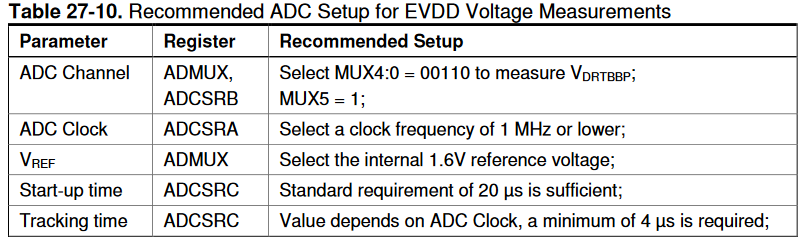
\includegraphics[scale=0.60]{images/Einstellungen}
	\caption{Konfiguration zur Messung der Spannung}
	\label{img:Konfiguration}
\end{figure}

\begin{figure}[!h]
	\centering
	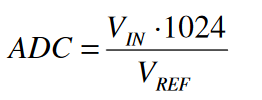
\includegraphics[scale=0.60]{images/Formel}
	\caption{Umrechnung}
	\label{img:Formel}
\end{figure}



\subsection{Stipe Knez}
Vergangene Woche Stand das Optimieren dreier Punkte bezüglich des Backends im Vordergrund. Das erste Problem, das behoben werden sollte war, dass wir in unserem Quellcode den COM-Port, über den das ZigBee Modul die Daten sendet, „gehardcoded“ war. Dies führte natürlich zu Problemen (bzw. einem Server crash), wenn man versucht hat, die Anwendung auf anderen Computern zu starten, da der COM-Port, über den das ZigBee Modul seine Daten schickt, ein anderer war. Dieses Problem haben wir durch das Programmieren einer „Port suchen“-Funktion gelöst, die anhand von spezifischen Daten wie „manufacturer“ und „vendor Id“ rausfiltert, an welchem COM-Port das Zigbee Modul angeschlossen ist und dann dementsprechend diesen zum Datenempfang verwendet.

Nachdem dieses Problem gelöst war, ging es an die Lösung eines Weiteren. Der Server stürzte immer dann ab, wenn vor dem Start des Backends kein Zigbee Modul angeschlossen war. Um dieses Problem zu lösen, integrierten wir des Weiteren eine Funktion, die die „Port suchen“-Funktion in einem bestimmten Intervall so lange ausführt, bis ein Modul angeschlossen und somit ein Port gefunden wird.

Die letzte Komplikation, die noch übrig blieb, war, dass der Empfang der Daten des ZigBee Moduls nicht mehr funktioniert hat, sobald man das Modul ausgesteckt und wieder angesteckt hat, während das Backend und somit der Server liefen. Stattdessen sollte es so sein, dass beim erneuten Anstecken das Modul wieder erkannt wird und der Datenempfang normal weiterläuft. Diese Funktionalität wurde dann auch umgesetzt durch das integrierten eines zusätzlichen „event listeners“, der im Fall eines „close“ Events (abstecken des Moduls mit daraus resultierendem disconnect) die im vorherigen Absatz erwähnte „Port suchen“-Funktion wieder im vorher erwähnten Intervall ausführt, bis ein erneutes anstecken des Moduls stattfindet.


\subsection{Lucas Merkert}
In dieser Woche habe ich ein wenig weniger gemacht, da ich mit der Fertigstellung eines anderen Projekts beschäftigt war. Es wurde vor allem das weitere Vorgehen besprochen und eine Anpassung des Dashboards Konzepts vorgenommen. Zudem wurde die Dokumentation angefangen und ein besser lesbares Zustandsdiagramm erstellt.

\subsection{Achim Glaesmann}


\subsection{Max-Rene Konieczka}
Für die vergangene Woche war vorgesehen, die gesendeten Daten in einem Live-Graph anzuzeigen. Allerdings stand zu diesem Zeitpunkt noch nicht ganz fest, wie genau das Dashboard aussehen soll. Daher wurde sich zunächst noch um die Struktur gekümmert. Es werden vier Diagramme zu sehen sein, um die Werte von Temperatur, CO2, relativer Luftfeuchte sowie der TVOC anzuzeigen. Im Verlauf dieser Woche wird sich nun hauptsächlich um das Anzeigen der Daten gekümmert. 

\subsection{Can Cihan Nazlier}
Diese Woche gab es einige Serverseitige und CLientseitige bugfixes. Es wurde besprochen wie die Ampel schalten soll und nach welchen Werten man geht. Der Server fällt nicht mehr aus wenn kein zigbee set dran ist. Es wurde neue Endpoints fürs dashboard erstellt.

\printbibliography
%----------------------------------------------------------------------------
% Bibliography
%----------------------------------------------------------------------------	

\end{document}
